\documentclass{article}
\usepackage{polski}
\usepackage[utf8]{inputenc}
\usepackage{amsmath}
\usepackage{amssymb}
\usepackage[dvipsnames]{xcolor}
\usepackage{tikz} 
\renewcommand{\labelitemi}{$\blacktriangleright$}

\begin{document}


\title{Sieci komputerowe - Ćwiczenia nr 1}
\author{Artur Bieniek}

\maketitle

\section*{1.}
Dla każdego z podanych poniżej adresów IP w notacji CIDR określ, czy jest to adres sieci, adres
rozgłoszeniowy czy też adres komputera. W każdym przypadku wyznacz odpowiadający mu adres
sieci, rozgłoszeniowy i jakiś adres IP innego komputera w tej samej sieci.
\begin{itemize}
    \item \texttt{10.1.2.3/8 = 00001010.\colorbox{Orange}{000000001.00000010.00000011}}
    \newline \textbf{Sieć:} \texttt{10.0.0.0/8}
    \newline \textbf{Broadcast:} \texttt{10.255.255.255/8}
    \newline \textbf{Adres IP:} \texttt{10.1.2.4/8}

    \item \texttt{156.17.0.0/16 = 10011100.00010001.\colorbox{Orange}{00000000.00000000}}
    \newline \textbf{Sieć:} \texttt{156.17.0.0/16}
    \newline \textbf{Broadcast:} \texttt{156.17.255.255/16}
    \newline \textbf{Adres IP:} \texttt{156.17.0.1/16}

    \item \texttt{99.99.99.99/27 = 01100011.01100011.01100011.011\colorbox{Orange}{00011}}
    \newline \textbf{Sieć:} \texttt{99.99.99.96/27}
    \newline \textbf{Broadcast:} \texttt{99.99.99.127/27}
    \newline \textbf{Adres IP:} \texttt{99.99.99.97/16}

    \item \texttt{156.17.64.4/30 = 10011100.00010001.01000000.000001\colorbox{Orange}{00}}
    \newline \textbf{Sieć:} \texttt{156.17.64.4/30}
    \newline \textbf{Broadcast:} \texttt{156.17.64.7/30}
    \newline \textbf{Adres IP:} \texttt{156.17.64.5/30}

    \item \texttt{123.123.123.123/32 = 01111011.01111011.01111011.01111011}
    \newline \textbf{Sieć:} \texttt{123.123.123.123/32}
    \newline \textbf{Broadcast:} \texttt{123.123.123.123/32}
    \newline \textbf{Adres IP:} \texttt{123.123.123.123/32} - dyskusyjna sprawa, bo według slajdów z wykładu to nie może być adres komputera w sieci
\end{itemize}

\section*{2.}
Podziel sieć 10.10.0.0/16 na 5 rozłącznych podsieci, tak aby każdy z adresów IP z sieci 10.10.0.0/16 był w jednej z tych 5 podsieci. Jak zmieniła się liczba adresów IP możliwych do użycia przy adresowaniu komputerów? Jaki jest minimalny rozmiar podsieci, który możesz uzyskać w ten sposób?
\newline
\textbf{Rozwiązanie:}
Sieci:
\begin{itemize}
    \item \texttt{10.10.0.0 - 10.10.31.255 /19}
    \item \texttt{10.10.32.0 - 10.10.63.255 /19}
    \item \texttt{10.10.64.0 - 10.10.95.255 /19}
    \item \texttt{10.10.96.0 - 10.10.127.255 /19}
    \item \texttt{10.10.128.0 - 10.10.255.255 /17}
\end{itemize}
Liczba adresów IP jest taka sama, ale ponieważ odejmujemy adres sieci i adres rozgłoszeniowy dla każdej sieci, to liczba adresów jest o 10 mniejsza. Minimalny rozmiar podsieci wynosi 4096, z czego użyteczne 4094. Jest tak ponieważ dzieląc maskę \texttt{/16} 5 razy uzyskamy minimalnie maskę 20, co daje $2^12=4096$. 

\section*{3.}
Tablica routingu zawiera następujące wpisy (podsieć $\rightarrow$ dokąd wysłać)
\begin{itemize}
    \item 0.0.0.0/0 $\rightarrow$ do routera A
    \item 10.0.0.0/23 $\rightarrow$ do routera B
    \item 10.0.2.0/24 $\rightarrow$ do routera B
    \item 10.0.3.0/24 $\rightarrow$ do routera B
    \item 10.0.1.0/24 $\rightarrow$ do routera C
    \item 10.0.0.128/25 $\rightarrow$ do routera B
    \item 10.0.1.8/29 $\rightarrow$ do routera B
    \item 10.0.1.16/29 $\rightarrow$ do routera B
    \item 10.0.1.24/29 $\rightarrow$ do routera B
\end{itemize}
Napisz równoważną tablicę routingu zawierającą jak najmniej wpisów.
\newline \textbf{Rowziązanie}
\begin{itemize}
    \item \texttt{0.0.0.0/0} $\rightarrow$ do routera A
    \item \texttt{10.0.0.0/22} $\rightarrow$ do routera B
    \item \texttt{10.0.1.0/24} $\rightarrow$ do routera C
    \item \texttt{10.0.1.8/28} $\rightarrow$ do routera B
    \item \texttt{10.0.1.24/29} $\rightarrow$ do routera B
\end{itemize}

\section*{4.}
Wykonaj powyższe zadanie dla tablicy
\begin{itemize}
    \item \texttt{0.0.0.0/0} $\rightarrow$ do routera A
    \item \texttt{10.0.0.0/8} $\rightarrow$ do routera B
    \item \texttt{10.3.0.0/24} $\rightarrow$ do routera C
    \item \texttt{10.3.0.32/27} $\rightarrow$ do routera B
    \item \texttt{10.3.0.64/27} $\rightarrow$ do routera B
    \item \texttt{10.3.0.96/27} $\rightarrow$ do routera B
\end{itemize}
\textbf{Rowziązanie}
\begin{itemize}
    \item \texttt{0.0.0.0/0} $\rightarrow$ do routera A
    \item \texttt{10.0.0.0/8} $\rightarrow$ do routera B
    \item \texttt{10.3.0.0/27} $\rightarrow$ do routera C
    \item \texttt{10.3.0.128/25} $\rightarrow$ do routera C
\end{itemize}

\section*{5.}
Jak uporządkować wpisy w tablicy routingu, żeby zasada najlepszego dopasowania odpowiadała wyborowi „pierwszy pasujący” (tj. przeglądaniu tablicy od początku do końca aż do momentu napotkania dowolnej pasującej reguły)? Odpowiedź uzasadnij formalnie.
\newline \textbf{Rozwiązanie:} \newline
Wystarczy posortować wpisy nierosnąco po maskach sieci, wtedy wpisy z tą samą maską podsieci muszą być rozłączne (o ile nie muszą zawsze być). Z wykładu: \textbf{Jeśli więcej niż jedna reguła pasuje, wybierana jest ta, która jest najdłuższym prefiksem (najbardziej "konkretna reguła")}. Tak więc jeśli posortujemy reguły po długości prefiksu, to najbardziej pasująca reguła będzie rozpatrywana jako pierwsza.

\section*{6.}
W podanej niżej sieci tablice routingu budowane są za pomocą algorytmu wektora odległości. Pokaż (krok po kroku), jak będzie się to odbywać. W ilu krokach zostanie osiągnięty stan stabilny?
\newline
\begin{tabular}{ |c|c|c|c|c|c| }
    \hline
    & A & B & C & D & E \\ \hline
    SU & 1 & 1 &  &  &  \\ \hline
    SW &  & 1 &  & 1 &  \\ \hline
    SX &  & 1 & 1 &  &  \\ \hline
    SY &  &  &  & 1 & 1 \\ \hline
    SZ &  &  & 1 & 1 &  \\ 
    \hline
\end{tabular}
\newline
\begin{tabular}{ |c|c|c|c|c|c| }
    \hline
    & A & B & C & D & E \\ \hline
    SU & 1 & 1 & 2 (via B) & 2 (via B) &  \\ \hline
    SW & 2 (via B) & 1 & 2 (via B) & 1 & 2 (via D) \\ \hline
    SX & 2 (via B) & 1 & 1 & 2 (via C) &  \\ \hline
    SY &  & 2 (via D) & 2 (via D) & 1 & 1 \\ \hline
    SZ &  & 2 (via C) & 1 & 1 & 2 (via D) \\ 
    \hline
\end{tabular}
\newline
\begin{tabular}{ |c|c|c|c|c|c| }
    \hline
    & A & B & C & D & E \\ \hline
    SU & 1 & 1 & 2 (via B) & 2 (via B) & 3 (via D) \\ \hline
    SW & 2 (via B) & 1 & 2 (via B) & 1 & 2 (via D) \\ \hline
    SX & 2 (via B) & 1 & 1 & 2 (via C) & 3 (via D) \\ \hline
    SY & 3 (via B) & 2 (via D) & 2 (via D) & 1 & 1 \\ \hline
    SZ & 3 (via B) & 2 (via C) & 1 & 1 & 2 (via D) \\ 
    \hline
\end{tabular}

\section*{7.}
Załóżmy, że w powyższej sieci tablice routingu zostały już zbudowane. Co będzie się działo (krok po kroku), jeśli zostanie dodana sieć SQ łącząca routery A i E?
\newline
\begin{tabular}{ |c|c|c|c|c|c| }
    \hline
    & A & B & C & D & E \\ \hline
    SU & 1 & 1 & 2 (via B) & 2 (via B) & 3 (via D) \\ \hline
    SW & 2 (via B) & 1 & 2 (via B) & 1 & 2 (via D) \\ \hline
    SX & 2 (via B) & 1 & 1 & 2 (via C) & 3 (via D) \\ \hline
    SY & 3 (via B) & 2 (via D) & 2 (via D) & 1 & 1 \\ \hline
    SZ & 3 (via B) & 2 (via C) & 1 & 1 & 2 (via D) \\ \hline
    SQ & 1 &  &  &  & 1 \\
    \hline
\end{tabular}
\newline
\begin{tabular}{ |c|c|c|c|c|c| }
    \hline
    & A & B & C & D & E \\ \hline
    SU & 1 & 1 & 2 (via B) & 2 (via B) & 2 (via A) \\ \hline
    SW & 2 (via B) & 1 & 2 (via B) & 1 & 2 (via D) \\ \hline
    SX & 2 (via B) & 1 & 1 & 2 (via C) & 3 (via D) \\ \hline
    SY & 2 (via E) & 2 (via D) & 2 (via D) & 1 & 1 \\ \hline
    SZ & 3 (via B) & 2 (via C) & 1 & 1 & 2 (via D) \\ \hline
    SQ & 1 & 2 (via A) & 3 (via D) & 2 (via E) & 1 \\
    \hline
\end{tabular}

\section*{8.}
W przedstawionej poniżej sieci uszkodzeniu ulega połączenie między routerami D i E . Załóżmy,
że w sieci działa algorytm wektora odległości wykorzystujący technikę zatruwania ścieżki zwrotnej
(poison reverse). Pokaż — opisując krok po kroku jakie komunikaty są przesyłane między routerami
— że może powstać cykl w routingu.
\newline
\textbf{Rozwiązanie:}
\begin{itemize}
    \item Router D wysyła do B i C informację, że jego ścieżka do E ma długość $\infty$.
    \item Router A wysyła do B, że ma do E ścieżkę długości 3 via C.
    \item Router B wysyła do D, że ma do E ścieżkę długości 4 via A.
    \item Router D wysyła do C, że ma do E ścieżkę długości 5 via B.
\end{itemize}
I tak dalej... - zliczanie do nieskończoności.

\section*{9.}
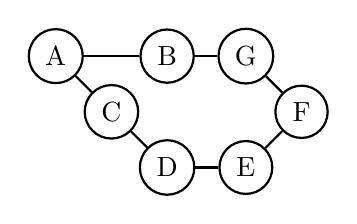
\begin{tikzpicture}[thick, main/.style = {draw, circle}] 
    \node[main] (1) {A};
    \node[main] (3) [below right of=1] {C};
    \node[main] (4) [below right of=3] {D};
    \node[main] (2) [above right of=3] {B};
    \node[main] (5) [right of=4] {E};
    \node[main] (6) [above right of=5] {F};
    \node[main] (7) [above left of=6] {G};
    \draw (1) -- (3);
    \draw (3) -- (4);
    \draw (4) -- (5);
    \draw (5) -- (6);
    \draw (6) -- (7);
    \draw (7) -- (2);
    \draw (1) -- (2);
\end{tikzpicture}
\newline Schemat powstania cyklu:
\begin{itemize}
    \item A i B tracą połączenie między sobą 
    \item C i G są powiadamiane o utracie połączenia AB
    \item D wysyła pakiet do B, najkrótszą ścieżką czyli przez C
    \item C zwraca ten pakiet spowrotem do D, bo wie że nie ma już tam drogi i najkrótsza droga prowadzi przez D
    \item Jest cykl i w teorii mogłyby sobie ten pakiet przesyłać w nieskończoność, w praktyce raczej prędko D dostanie komunikat o utracie łącza AB i wybierze inną trasę
\end{itemize}

\section*{10.}
Załóżmy, że sieć składa się z łączy jednokierunkowych (tj. łącza w sieci tworzą graf skierowany) i nie zawiera cykli. Rozważmy niekontrolowany algorytm „zalewający” sieć jakimś komunikatem: komuni- kat zostaje wysłany początkowo przez pewien router; każdy router, który dostanie dany komunikat przesyła go dalej wszystkimi wychodzącymi z niego krawędziami. Pokaż, że istnieją takie sieci z n routerami, w których przesyłanie informacji zakończy się po czasie $2^{\Omega(n)}$. Zakładamy, że przez jedno łącze można przesłać tylko jeden komunikat naraz, a przesłanie go trwa jednostkę czasu.
\newline \textbf{Rozwiązanie:} Poniższy graf potrafi podwoić liczbę komunikatów. \newline
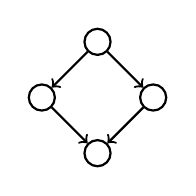
\begin{tikzpicture}[thick, main/.style = {draw, circle}] 
    \node[main] (1) {};
    \node[main] (2) [below left of=1] {};
    \node[main] (3) [below right of=1] {};
    \node[main] (4) [below right of=2] {};
    \draw[->] (1) -- (2);
    \draw[->] (1) -- (3);
    \draw[->] (2) -- (4);
    \draw[->] (3) -- (4);
\end{tikzpicture}
\newline
Powtarzając ten graf n razy, za każdym razem łącząc początek z końcem, mamy 4n wierzchołków, w ostatnim takim rombie wysłanie wiadomości zajmie $2^n$ jednostek czasu. Mamy zatem $n$ wierzchołków, a przesyłanie komunikatu zakończy się w czasie $2^{n/4} = 2^{\Omega(n)}$.

\end{document}